\section{Άσκηση 1}

Στην αρχή έχω τα απαραίτητα imports για \texttt{numpy}, \texttt{scipy} και
\texttt{matplotlib}:

\lstinputlisting[firstline=1, lastline=8]{ex1/ex1.py}

Η συνάρτηση και οι 2 πρώτες παράγωγοι
ορίζονται και γίνεται το plot της $f(x)$:

\lstinputlisting[firstline=9, lastline=24]{ex1/ex1.py}
\begin{center}
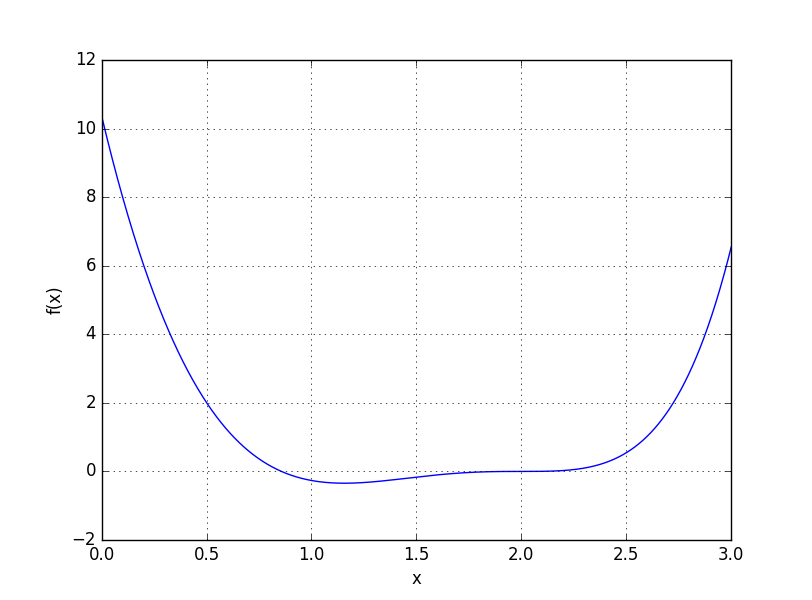
\includegraphics[width=\linewidth, height=9cm]{ex1/plot.png}
\end{center}

Καθώς η άσκηση δεν το απαιτεί δεν υπάρχουν έλεγχοι για σφάλματα
ούτε συνθήκες τερματισμού σε περίπτωση που δεν υπάρχουν ρίζες.
\subsection{Διχοτόμηση}
Ακολουθεί η συνάρτηση για διχοτόμηση:
\lstinputlisting[firstline=26, lastline=41]{ex1/ex1.py}

Απλά γίνετε η εγαρμογή του θεωρήματος για
$N = {{\ln{(b-a)} - \ln{(error)}}\over{\ln{2}}}$ φορές
\newpage
\subsection{Newton-Raphson}
Στην συνέχεια έχω τη συνάρτηση για την μέθοδο Newton-Raphson:
\lstinputlisting[firstline=42, lastline=54]{ex1/ex1.py}

Εδώ αρχικοποιώ τον πίνακα \texttt{temp\_l} με την τιμή
εισόδου της συνάρτησης και το αποτέλεσμα μιας πρώτης εφαρμογής της
αναδρομικής συνάρτησης $$f(x_{n}) = f(x_{n-1}) - {{f(x_{n-1})} \over {f'(x_{n-1})}}$$
Στην συνέχεια με τον έλεγχο στο while η συνάρτηση θα τρέχει μέχρι να
επιτευχθεί η επιθυμιτή ακρίβεια (6 δεκαδικά ψηδία)

Επιστρέφω την ρίζα, τον αριθμό επαναλήψεων και το σημείο εκκίνησης.

\subsection{Τέμνουσα}
Ακολουθέι η συνάρτηση της μεθόδου της τέμνουσας:
\lstinputlisting[firstline=55, lastline=68]{ex1/ex1.py}

Η συνάρτηση είναι αντίστοιχη με αυτή της Newton-Raphson.
Χρειάζεται δύο αρχικές τιμές, και για να γίνει ο έλεγχος του \texttt{while},
υπολογίζω και την τρίτη σύμφωνα με την αναδρομική συνάρτηση
$$x_{n+1} = x_n - {{f(x_n)(x_n - x_{n-1})} \over {f(x_n) - f(x_{n-1})}}$$
Ο έλεγχος είναι ο ίδιος με την Newton-Raphson για να πετύχω τα
6 δεκαδικά ψηφία

Επιστρέφω την ρίζα, τον αριθμό επαναλήψεων καθως και τις 2 αρχικές τιμές.

\subsection{Αποτελέσματα}
Ακολουθεί η έξοδος του προγράμματος όταν το τρέχω με τις
κατάλληλες αρχικές τιμές (βασισμένες στο διάγραμμα την συνάρτησης):

\begin{lstlisting}[language=C, mathescape=true]
$\dollar$ python ex1/ex1.py
++++ Bisection ++++

Root in [0.00,1.50] after 22 loops: f(0.857143) = -0.000000

Root in [1.50,3.00] after 22 loops: f(2.000004) = 0.000000

++++ Newton - Raphson ++++

Starting at 1.00:
after 5 iterations the root is: f(0.857143) = 0.000000

Starting at 3.00:
after 14 iterations the root is: f(2.005224) = 0.000000

++++ Interpolation ++++

Root found in [0.70,0.90] after 10 iterations:
f(0.857143) = 0.000000

Root found in [1.70,2.10] after 20 iterations:
f(2.004977) = 0.000000
\end{lstlisting}

\newpage
\subsection{Παρατηρήσεις}
Στο διάγραμμα που ακολουθεί βλέπουμε τις επαναλήψεις που
χρειάζετε η μέθοδος Newton-Raphson σε σχέση με την αρχική τιμή
που δίνεται

\begin{center}
  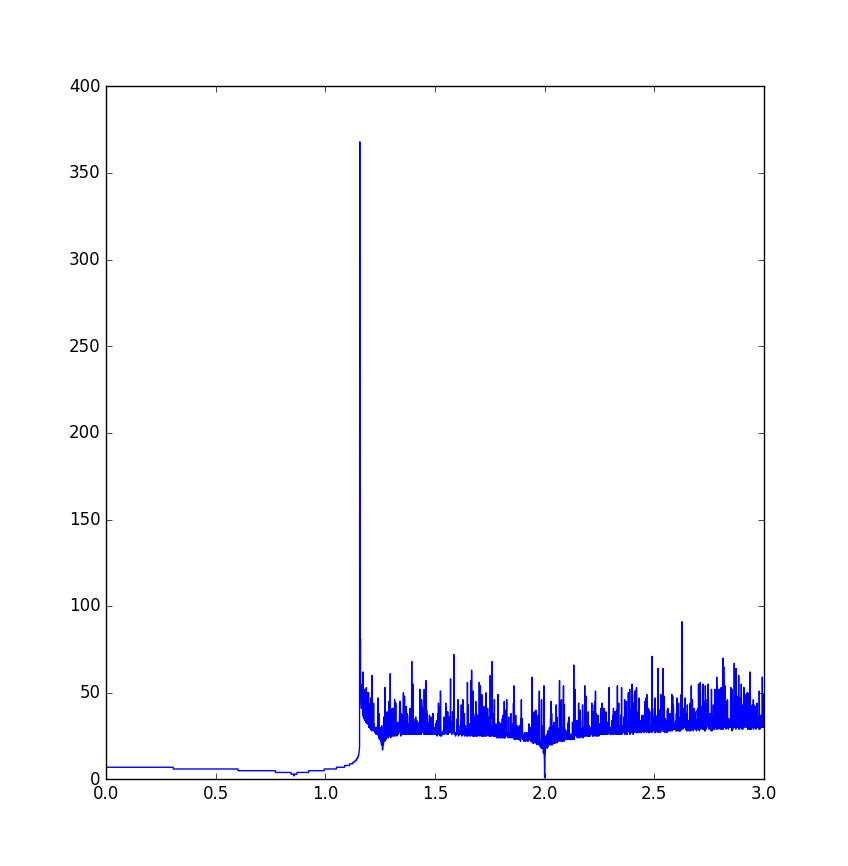
\includegraphics[scale = 0.7]{ex1/starting_point-loops.png}
\end{center}

Παρατηρώ οτι για την ρίζα στο $0.857143$ η μέθοδος συγκλίνει τετραγωνικά
ενώ για την ρίζα στο $2.000004$ θέλει εμφανώς περισσότερες επαναλήψεις.

Συγκρίνοντας αυτό το διάγραμμα με το plot της συνάρτησης στην 1η σελίδα
παρατηρώ οτι η ταχύτητα σύγκλισης στην πρώτη ρίζα είναι μεγάλη γιατι η
συνάρτηση διατηρεί την ίδια κυρτώτητα ενώ στην δεύτερη η συνάρτηση αλλάζει.

Καθώς η μέθοδος N-R χρησιμοποιεί την κλίση της παραγόγου για να βρεί το
επόμενο $x$ στην αναδρομή, όταν η κυρτώτητα αλλάζει γύρω απο την ρίζα
ο αλγόριθμος ταλαντώνετε και αργεί να συγκλίνει σε έναν αριθμό που να ικανοποιεί
το σφάλμα που θέσαμε.
%%% Local Variables:
%%% mode: latex
%%% TeX-master: "../master"
%%% End:
